\chapter{Fortran90の応用1〜数値計算の高速化〜}

%以上のように, 
コンピュータによる数値計算は, 手計算では解を求めることができないような複雑な問題であっても, 
計算誤差の範囲内で近似的に解くことができ, 現代の科学技術を支える非常に強力な手段である.  
しかしながら, 多くの場合, すぐに計算量が膨大になり, 現実的な時間内に計算が終わらなくなってしまう. 
それを克服するためには, アルゴリズムを工夫して意味のない計算を省略するなどして, 
計算時間を短くすることが必要である. 

この章では``素数の探索''という簡単な例を用いて, 数値計算の高速化を体験する. 


\section{素数探索}
素数とは1と自分以外に約数をもたない自然数のことである.
ここでは, 計算機を用いて膨大な数の素数をいかに速く求めるかを目指す. 

\subsection*{$<$演習課題4.1$>$}
\begin{enumerate}
\item ある自然数$n$を与え, それを$n-1$までの自然数で割り算することにより, 
$n$が素数かどうかを判定するプログラムを作成せよ. 
(ヒント: 余りを計算する関数\verb|mod|を利用する)
\item 上記のプログラムをサブルーチン化し, 100,000番目の素数の値を求めるプログラムを作成せよ. 
\end{enumerate}

\subsection{実行速度の計測}
次に, 上で作成したプログラムの高速化に取り組む. 

プログラムの高速化を行うためには, やみくもに試行錯誤を行なうのではなく, 
どの計算に時間がかかっているか(ホットスポットと呼ばれる)を調べ, 
多くの計算時間が費やしている部分を重点的に改善することが必要である. 

プログラムの実行時間は, \verb|system_clock|関数により得ることができる.
以下に, 計算時間を計測するプログラムの一例を示す. 

\lstinputlisting[caption={実行時間の測定. }, label=timing]{8_fortran5/codes/Timing.f90}


\subsection*{$<$演習課題4.2$>$}
\begin{enumerate}
\item 100,000番目の素数の探索にかかった時刻を計測するプログラムを作成せよ. 
\item $i$番目の素数の探索にかかった時間$t(i)$をグラフに描画し, 
その様子から素数探索にかかる時間の特徴を考察せよ. 
\item 上での考察を元にアルゴリズムを工夫して, 100,000番目の素数を探索する高速なプログラムを作成せよ.
\end{enumerate}







\begin{comment}
  \section{素数探索}

  以下にプログラム例を示す. 
  %TODO 実行時間を測れる例に変更する. 
  %TODO 特にわかりやすい例として, ファイルへの書き込みを毎回行っておく. 



  \section{Mandelbrot集合}
  Mandelbrot集合とは,
  \begin{equation}
  z_{n+1}=z_n^2+c, \ \ \ z_0=0
  \end{equation}
  という漸化式で定義される複素数列$z_n$が$n \to \infty$の極限で発散しないという
  条件を満たす複素数$c$の集合である.
  Mandelbrot集合はその一部が全体と相似であり, フラクタルと呼ばれる.

  $|z_n|>2$のとき, $|z_{n+1}/z_n|>1$となることが示されるので(証明略),
  複素数列が発散する条件はある$N$に対して$|z_N|>2$となることである.

  \begin{figure}[ht]
  \centering
  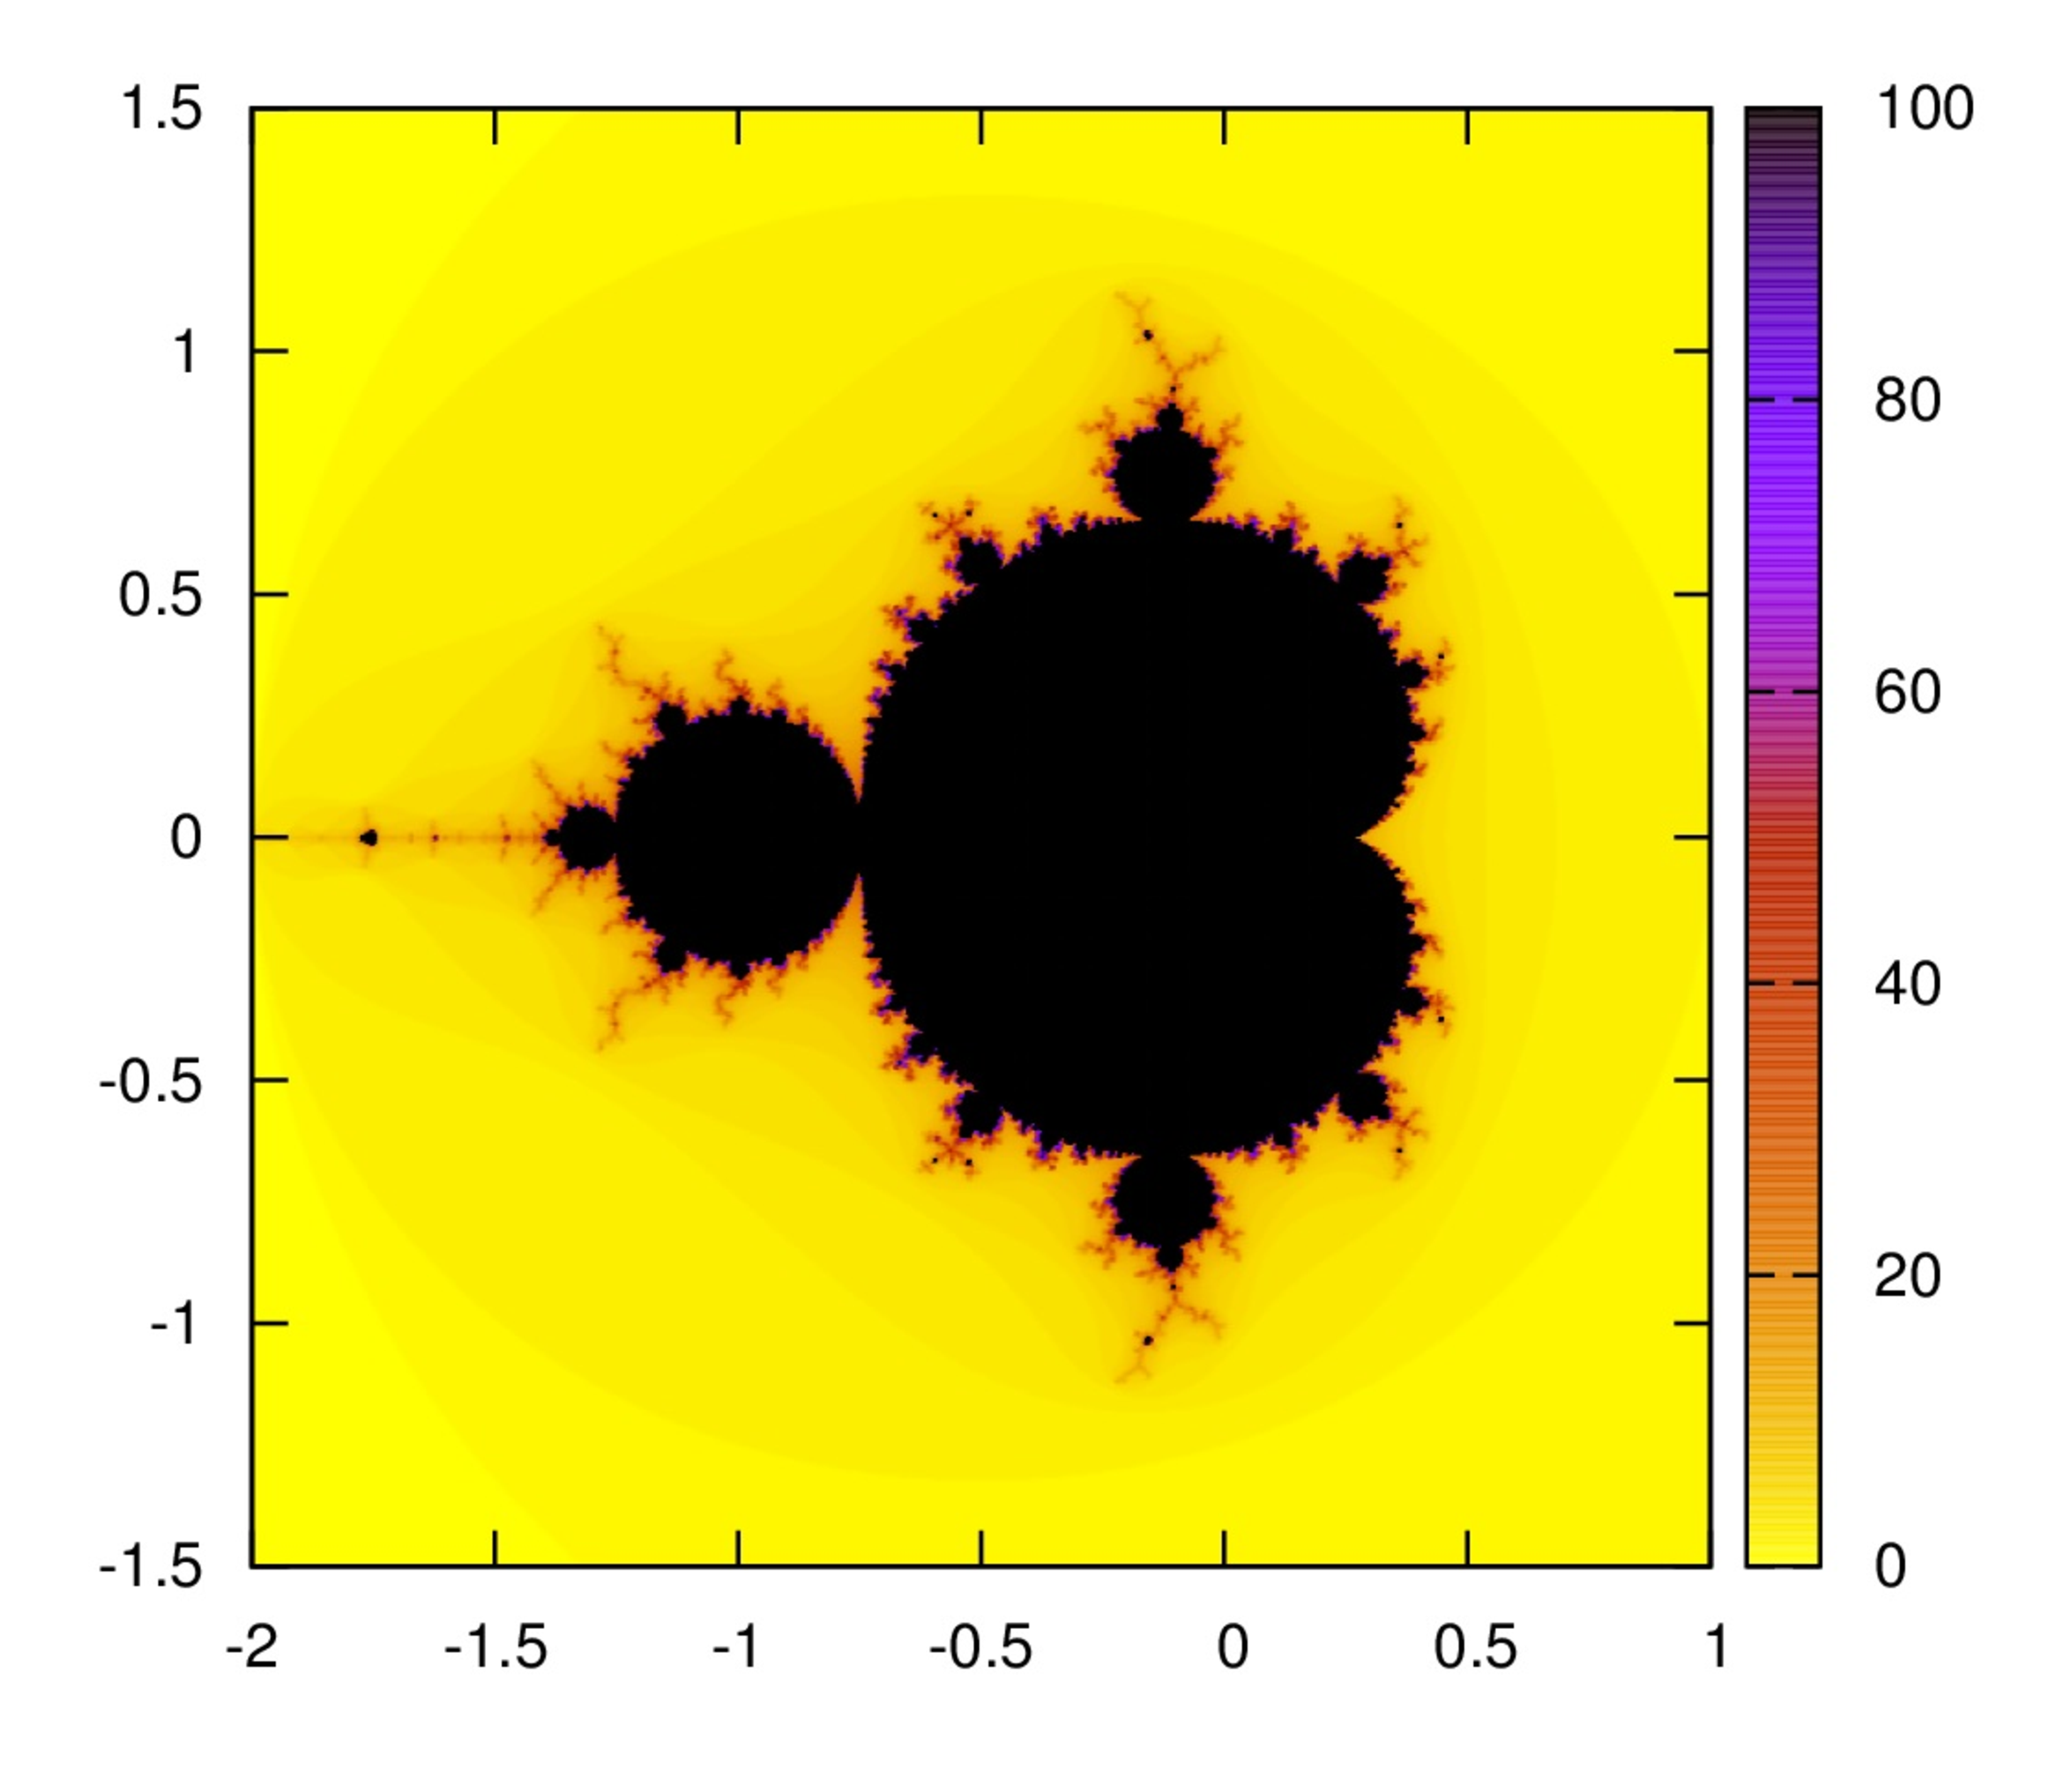
\includegraphics[width=0.75\linewidth]{9_fortran6/figs/mandel}
  \caption{Mandelbrot集合. }
  \end{figure}

  \subsection*{$<$演習課題$>$}
  \begin{enumerate}
  \item 複素数$c$を与え, $|z_N|>2$を満たす最初の$N$を出力するプログラムを作成せよ.
  \item 上のプログラムを改造して, $-2 \le \Re[c] \le 1, -1.5 \le \Im[c] \le 1.5$の範囲における$N$をファイルに出力せよ.
  また, 出力ファイルをカラーマップで描画せよ.
  \item 図形の一部を解像度を上げて再計算し, Mandelbrot集合がフラクタルであることを確かめよ.
  \end{enumerate}


\end{comment}
